\documentclass{article}
\usepackage[utf8]{inputenc}
\usepackage[portuguese]{babel}
\usepackage{amsmath}
\usepackage{physics}
\usepackage{amsmath}
\usepackage{tikz}
\usepackage{mathdots}
\usepackage{yhmath}
\usepackage{cancel}
\usepackage{color}
\usepackage{siunitx}
\usepackage{array}
\usepackage{multirow}
\usepackage{amssymb}
\usepackage{gensymb}
\usepackage{tabularx}
\usepackage{booktabs}

\usetikzlibrary{patterns}
\usetikzlibrary{shadows.blur}
\usetikzlibrary{shapes}

\title{Trabalho Final - PAA \\ Branch and Bound e Backtracking}
\author{Larissa Domingues Gomes - 650525 \\
Pedro Henrique Lima Carvalho - 651230}
\date{Novembro 2021}

\usepackage{natbib}
\usepackage{graphicx}

\begin{document}

\maketitle

\section{Branch and Bound}
\textit{Branch and Bound} é uma estratégia para desenvolvimento de algoritmos utilizada para problemas de otimização combinatória, ou seja, algoritmos que buscam encontrar uma solução ótima de maximização ou minimização em conjuntos finitos. 

\par Algoritmos que utilizam a abordagem de \textit{Branch and Bound} dividem o problema em problemas menores e os organiza em uma estrutura de árvore de estado, sendo assim, cada ramificação da árvore é considerada como um possível candidato a solução do problema. Para explorar cada ramificação da árvore, algoritmos de \textit{Busca em Largura} e \textit{Busca em Profundidade} podem ser utilizados. A cada nó visitado, um cálculo é realizado para encontrar o limite máximo ou mínimo que poderá resultar da exploração ramificações deste nó. Caso um possível resultado seja encontrado, esses limites deverão ser considerados para decidir se as ramificações podem ser exploradas a fim de encontrar um resultado melhor, ou o nó deverá ser descartado da solução. Geralmente, o tempo para que a solução ótima seja encontrada no pior caso é exponencial, isso ocorre principalmente em casos que todos os nós da árvore devem ser explorados. 

\par O algoritmo implementado neste trabalho que utiliza a técnica \textit{Branch and Bound} para resolver o famoso problema de minimização \textit{Travelling Salesperson}, que tem como objetivo encontrar o menor caminho de um grafo para que cada vértice seja visitado apenas uma vez, e ao final, deve-se retornar ao vértice de origem.
\begin{center}
\par 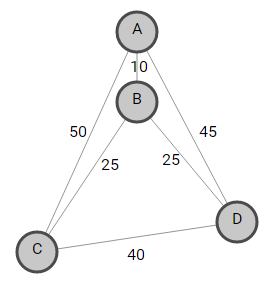
\includegraphics[width=5cm, height=5cm]{grafoTSP.png} \par
\end{center}

\par Tendo em vista o grafo acima, representado pela matriz: 
\begin{center}
\par 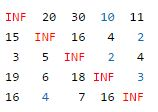
\includegraphics[width=5cm, height=5cm]{matriz1.jpg} \par
\end{center}

\par O primeiro passo do algoritmo, consiste em encontrar para cada linha e coluna da matriz do nó raiz o menor peso e subtrair o valor de cada elemento de sua respectiva linha ou coluna. Posteriormente, deve-se somar esses valores, assim o valor da redução é encontrado. O valor de redução representa o limite do menor valor que poderá ser encontrado como resultado do problema do caixeiro viajante, pois ele é a soma das menores arestas incidentes a cada vértice. A matriz resultante após o primeiro passo será:

\begin{center}
\par 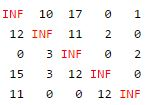
\includegraphics[width=5cm, height=5cm]{matriz2.jpg} \par
\end{center}

Após o processo feito no nó raiz, deve-se repetir o processo do cálculo de redução a cada nó da árvore de estados, com algumas modificações. Após escolher um nó filho para analisar o resultado do seu estado,todos elementos da coluna do nó pai e da linha do nó filho deve sem alterados para infinito, o elemento da posição (pai, filho) também deverá ter seu valor alterado, isso se deve para evitar retornar a esse vértices após visita-los.

Exemplo: visitar nó 2 a partir de 0. 

\begin{center}
\par 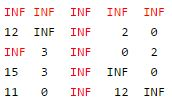
\includegraphics[width=5cm, height=5cm]{matriz3.jpg} \par
\end{center}

Após realizar a redução de linhas e colunas da matriz como no primeiro passo, o cálculo da redução será a soma dos menores elementos de cada linha e coluna + valor da aresta (pai, filho) na matriz de redução do pai + redução do estado anterior. O processo deverá ser repetido para cada nó visitado até os nós folha. Quando algum nó folha for alcançado, a redução calculada irá resultar no peso total do caminho percorrido. Uma árvore de soluções do grafo acima pode ser: 

\begin{center}
\par 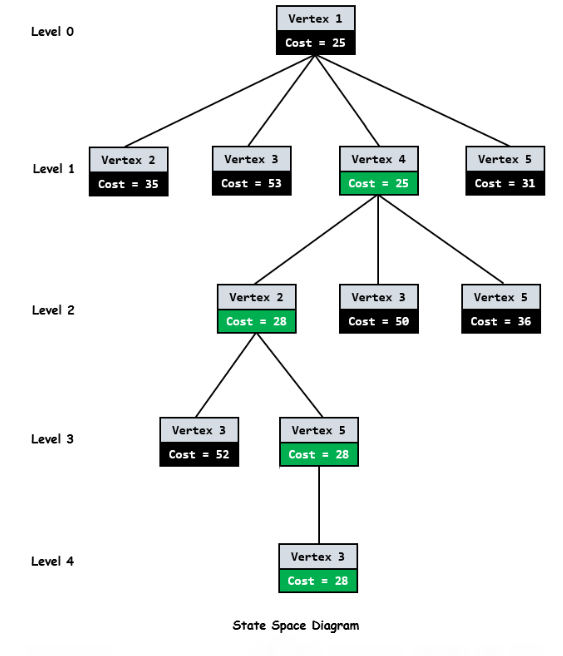
\includegraphics[width=8cm, height=11cm]{arvore.png} \par
\end{center}

Para explorar a árvore acima utilizou busca em profundidade para visitar seus respectivos nós, o resultado do \textit{Travelling Salesperson} para o grafo apresentado é 28. Observa-se que após o cálculo do nó folha que apresentou resultado 28, a busca foi interrompida, pois nenhum cálculo de redução dos nós anteriores apresentou valor menor que 28, logo não faria sentido continuar a busca. 





\section{Backtracking }
\textit{Backtracking} consiste em técnica de solução de problemas recursiva, que visa obter a solução de forma incremental. Utiliza-se uma árvore de estado, construída no modo DFS (Deep First Search), onde a recursão começa na raiz e explora o máximo possível cada ramo antes de voltar. No entanto, ao contrário de um algorítimo força bruta, a cada nível, testa-se a viabilidade da solução, encerrando aquele ramo e voltando caso seja inviável.
\par
A técnica pode ser utilizada para problemas de decisão, de otimização e de enumeração que tenham requisitos claros e bem definidos. No entanto, para problemas de decisão e otimização, outras técnicas como \textit{Programação Dinâmica} ou \textit{Programação Linear} têm desempenho superior, sendo mais aconselhado o uso de \textit{Backtracking} para problemas de enumeração.
\par
O exemplo escolhido para implementação foi o problema N-Queens: Em um tabuleiro de xadrez \(N\)x\(N\), deve-se posicionar \(N\) rainhas de forma que uma não consiga atacar a outra.
\par
O algorítimo inicia colocando uma rainha na primeira posição da primeira linha (1,1), desce na árvore e tenta posicionar, na segunda linha, uma rainha na primeira posição (2,1). Porém, ao contrário de um algorítimo força bruta, nesse momento já se verifica que as duas rainhas colocadas podem se atacar, o ramo é encerrado e retorna-se para o nó (1,1).
\par
Até a obtenção da primeira solução, a árvore de estado construída será a seguinte:

\begin{center}
\par 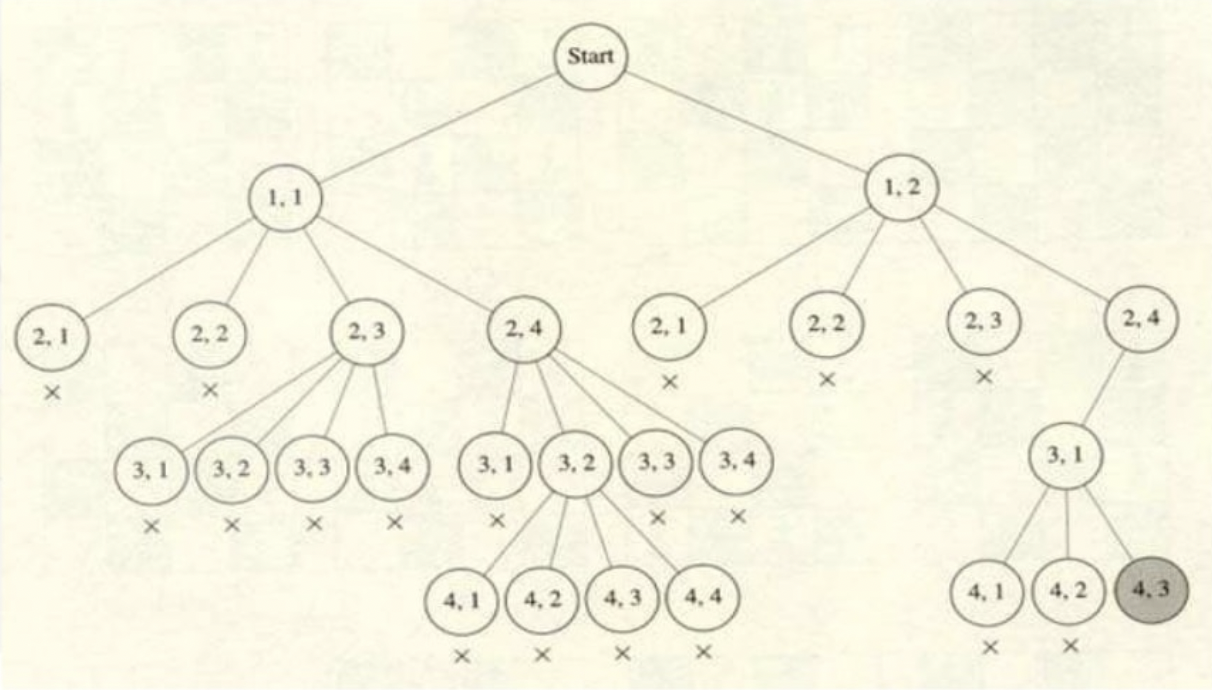
\includegraphics[width=10cm, height=6cm]{tree.png} \par
\end{center}

O que equivale ao seguinte posicionamento das rainhas:

\begin{center}
\par 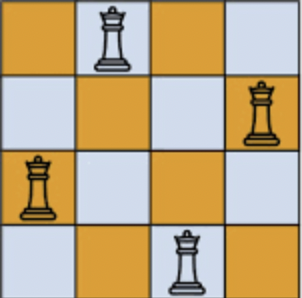
\includegraphics[width=6cm, height=6cm]{solution.png} \par
\end{center}


\section{Semelhanças e Diferenças}
A semelhança entre \textit{Backtracking} e \textit{Branch and Bound} é que ambas estratégias utilizam uma árvore de estados para explorar possíveis soluções e descartam ramificações que irão não retornar o melhor resultado.
\par
A principal diferença entre os dois algoritmos está na forma de exploração da árvore. \textit{Branch and Bound} permite explorar a árvore tanto com \textit{Busca em Largura}, quanto \textit{Busca em Profundidade}, garantido o retorno do melhor resultado. Por outro lado, a árvore só poderá ser explorada por \textit{Busca em Profundidade} em  algoritmos de \textit{Backtracking}, pois apenas com a \textit{Busca em Profundidade} será possível retornar ao ponto em que uma decisão errada foi tomada.
\par
Outra diferença muito marcante entre ambas estratégias é a função calculada em cada nó. Em \textit{Branch and Bound}, essa função tem como objetivo estabelecer o limite máximo ou mínimo que poderá ser alcançado a partir das ramificações de um nó, já em \textit{Backtracking}, o cálculo feito busca decidir se o nó selecionado é viável para resposta ou não. 
\par
A aplicação dos tipos algoritmos é outro ponto de divergência, \textit{Branch and Bound} é utilizado para problemas que envolvem otimização, retornando apenas uma solução, em contrapartida, \textit{Backtracking} é mais presente em algoritmos decisão, podendo oferecer múltiplas soluções.
\par
Tal como \textit{Branch and Bound}, a técnica de Programação Dinâmica também é utilizada para problemas de otimização. No entanto, a última se mostra uma ferramenta mais poderosa, vez que, além de encerrar ramificações fora dos limites, reaproveita cálculos já executados através de memoização. 
\par
Da mesma forma que a técnica de Divisão-e-Conquista, \textit{Branch and Bound} e \textit{Backtracking} são técnicas recursivas, que dividem o problema em problemas menores. Porém, enquanto as duas últimas adotam estratégias de eliminação de ramos, a Divisão-e-Conquista calcula todas as ramificações. 
\par
Por fim, cabe ressaltar que, enquanto \textit{Branch and Bound} e \textit{Backtracking} eliminam apenas as ramificações que, com certeza, não fazem parte da solução, a Abordagem Gulosa realiza uma escolha "míope", buscando otimizar o resultado com base, apenas, nas opções imediatas do momento. A otimização realizada por essa abordagem pode apresentar solução não ótima.

\end{document}